\chapterimage{apps.jpg}

\chapter{Layer 7: Application}\label{sec:layer7}

\begin{minipage}{0.4\linewidth}
\begin{center}
\begin{bytefield}{16}
\bitbox{16}{\color{color1} Layer 7: Application} \\
\bitbox{16}{Layer 4: Transport} \\
\bitbox{16}{Layer 3: Internet} \\
\bitbox{16}{Layer 2: Network (LAN)} \\
\bitbox{16}{Layer 1: Physical} \\
\end{bytefield}
\end{center}
\end{minipage}
\begin{minipage}{0.6\linewidth}
\begin{center}
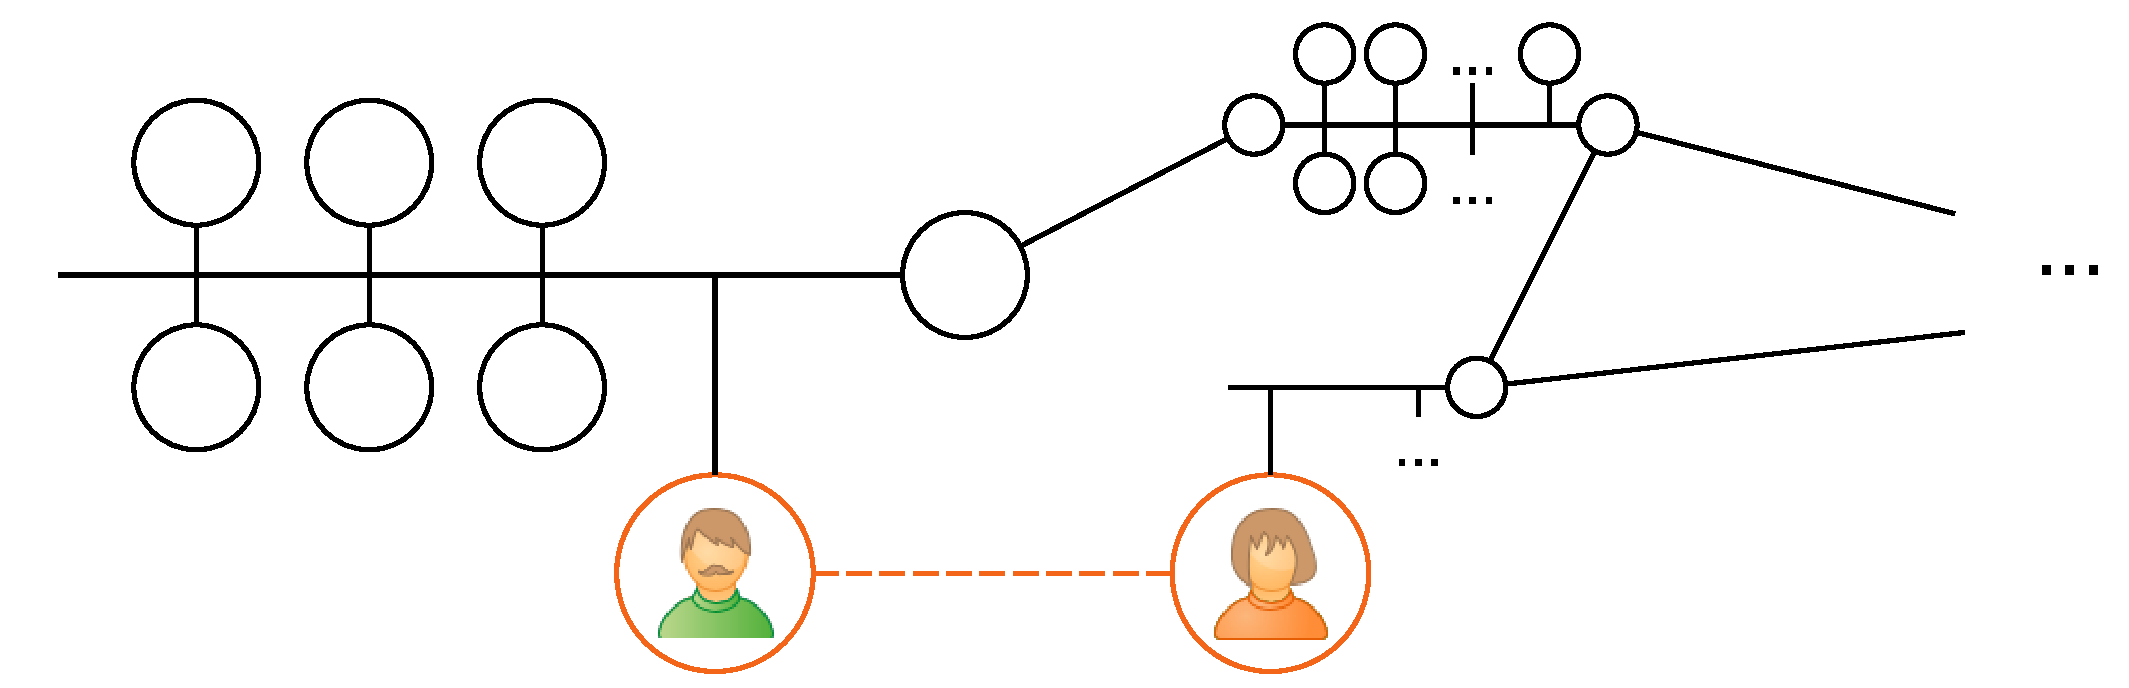
\includegraphics[width=\linewidth]{network_layer7.pdf}
\end{center}
\end{minipage}

The top layer of the TCP/IP network stack includes all applications 
that use TCP or UDP for transport. It is by far the one that contains 
the largest number of protocols, and where those protocols are more 
quickly created and replaced.

In addition to user apps, there are several auxiliary systems and protocols that 
help with configuration and operation of all hosts in the Internet. 
Some of the most critical are addressed in this chapter.

\section{DNS -- Domain Name System}

The \concept{DNS} protocol is responsible for translating \conceptRef{domain name}{domain names}
such as \otherBase{ietf.org} or\\\otherBase{cv.uab.cat} into \concept{IP}
addresses that can placed inside \conceptRef{datagram}{datagrams}.

DNS services are run on both \concept{TCP} and \concept{UDP}, \ie, both transport protocols
can be enabled. In both cases, port \otherBase{53} is used.

\subsection{Hierarchy}\label{sec:layer6:dns:hierarchy}

\begin{center}
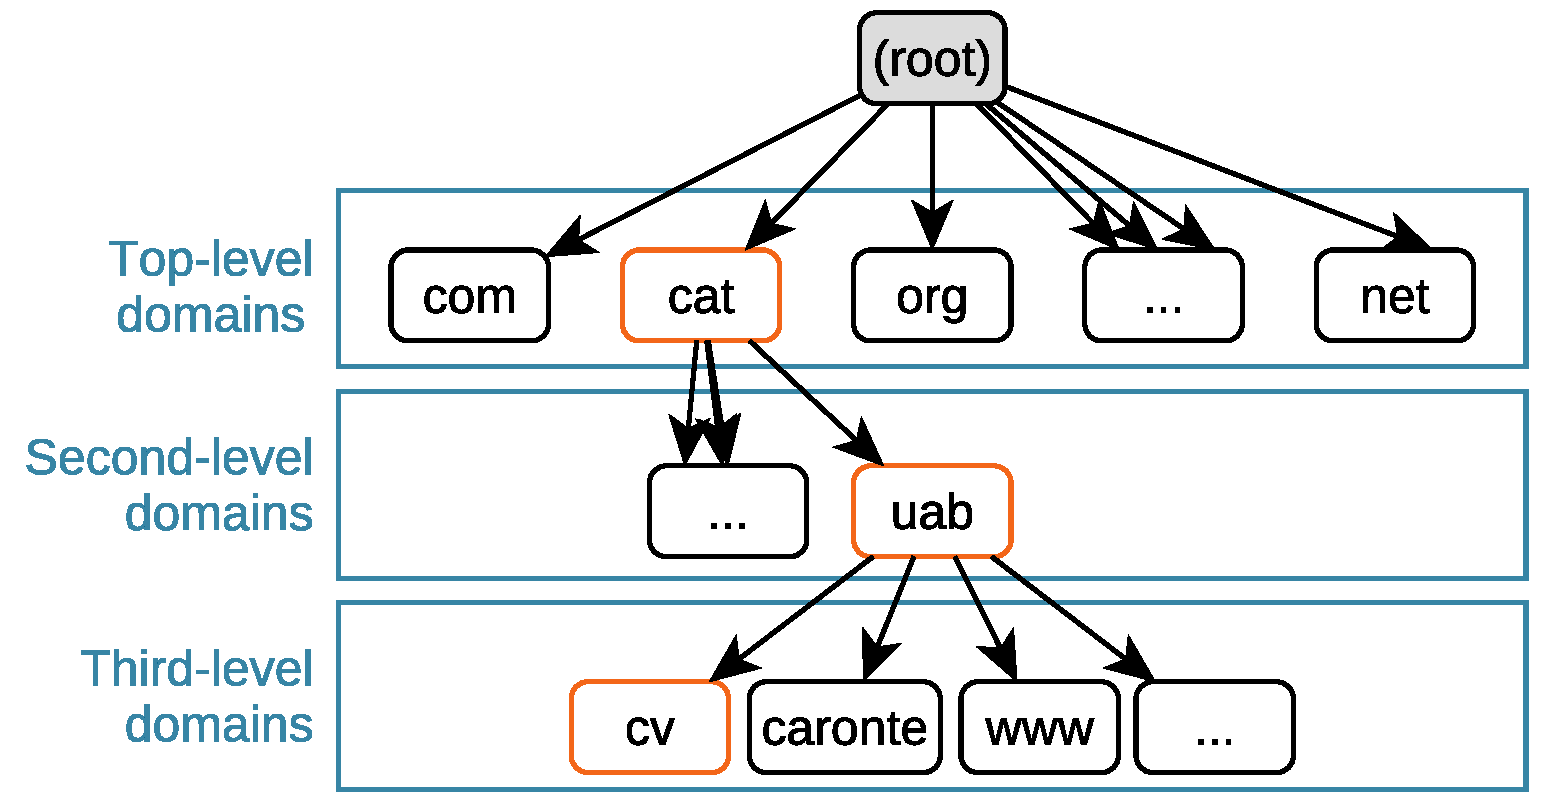
\includegraphics[width=0.65\linewidth]{dns_hierarchy.pdf}
\end{center}

Internet domain names are sequences of names separated by dots. 
These names are presented from the specific to the general in a hierarchical fashion.
For instance, in \otherBase{cv.uab.cat}, \otherBase{cv} belongs to \otherBase{uab.cat},
and \otherBase{uab} to \otherBase{cat}.
% 
The rightmost name, \eg, \otherBase{cat} or \otherBase{com} 
must be one of IANA's \conceptRef{top-level domain}{top-level domains}.

DNS servers are organized in the same hierarchical way as those domain names.
There are $13$ \concept{root DNS} servers (\inlineCode{Root-A} to \inlineCode{Root-M}),
which are responsible for all top-level domains.
You can ask any of them about \otherBase{com}, 
but also about \otherBase{su}, and they will know about them.

That does not mean that any root server knows about every domain \textit{under}
their top-level domain (\eg, \otherBase{uab.cat}): they just know about those 
\href{https://en.wikipedia.org/wiki/List_of_Internet_top-level_domains}{\underline{top-level domains}}.
(\eg, \otherBase{cat}).
% 
The job of the root DNS servers is to redirect you to another DNS server in charge 
of the \concept{top-level domain} you requested.
 
Similarly, the DNS servers responsible for \otherBase{cat} will know about 
any existing \otherBase{*.cat} domain (\eg, \otherBase{uab.cat}), 
but not about subdomains (\eg, \otherBase{cv.uab.cat}). 
% 
The job of those top-level domain DNS servers is to redirect you to 
other DNS servers \concept{authoritative} for the second-level domain 
requested (\eg, \otherBase{uab.cat}).
% 
Second-level domains can then structure their name \concept{zone} 
as desired, including any subdomain number and depth, as well as
the name to IP translation \textit{within} the zone of authority.

\begin{exercise}
Everyone uses DNS all the time. What would be the risks of having
a centralized name translation system instead of DNS's distributed nature.
\end{exercise}

\subsection{Records}

DNS can be seen as a distributed database with different types of entries
called \conceptRef{DNS record}{records}. The main ones are:

\begin{itemize}
\item[\textbf{A}:] An \concept{A} entry maps a domain name to an IPv4 address.
\item[\textbf{AAAA}:] An \concept{AAAA} entry maps a domain name to an IPv6 address.
\item[\textbf{NS}:] An \concept{NS} points to a DNS server that can help.
\item[\textbf{MX}:] A \concept{MX} entry provides the domain name of the email server 
  that handles messages for a domain.
\item[\textbf{CNAME}:] A \concept{CNAME} entry maps a domain name to another domain name.
\end{itemize}

Applications make \conceptRef{request}{requests} to DNS servers indicating the type 
of records they are interested in. Server \conceptRef{reply}{replies} may be for
the requested \concept{A} or \concept{MX} records, 
but the client may also receive a redirection to another DNS (\concept{NS}) 
or an alias to another domain name (\concept{CNAME}).

\subsection{Resolution}

The distributed and hierarchical nature if the DNS database makes it 
sometimes necessary to exchange multiple messages to satisfy a DNS \concept{query}.
 
For instance, Alice may perform a fully \concept{iterative} resolution all on her own.
The first two replies contain an \concept{NS} entry pointing to the next 
DNS server and the IP address of that DNS server, but not the IP address of the 
requested \otherBase{cv.uab.cat}.

\begin{center}
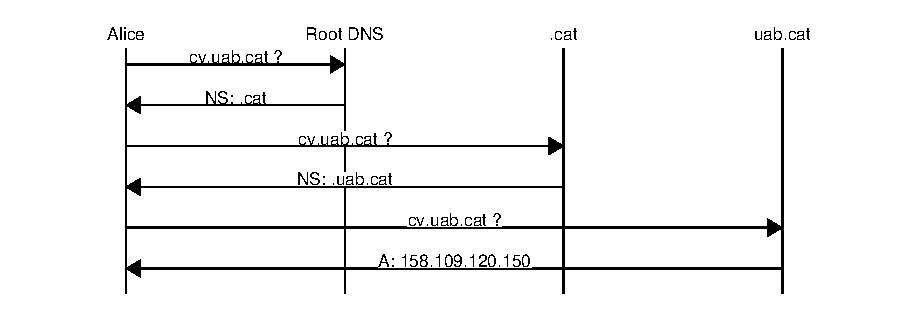
\includegraphics[width=\linewidth]{dns_iterative.eps}
\end{center}

Alice's internet provider (\concept{ISP}) or employer will likely offer DNS servers 
whose job is to receive Alice's requests and resolve them for her in a \concept{recursive} 
manner.

\begin{center}
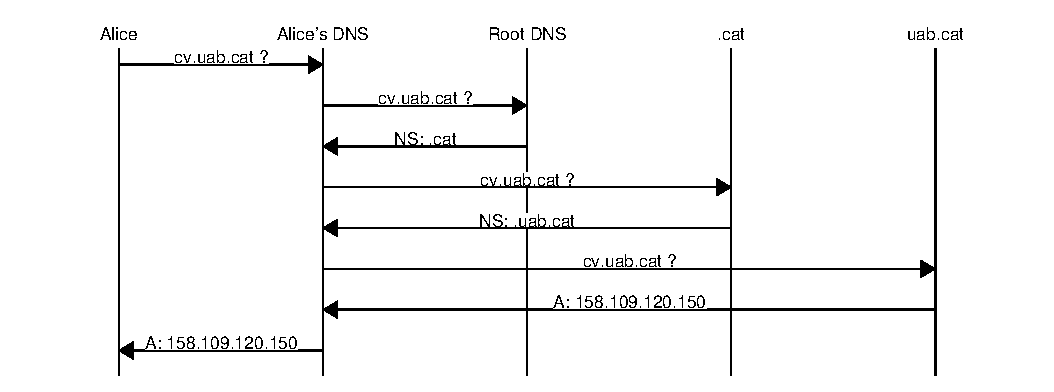
\includegraphics[width=1.05\linewidth]{dns_recursive.eps}
\end{center}

The combination of \concept{recursive} resolution and \concept{cache} tables makes
DNS a pretty efficient system with extremely high availability and low latency.

\begin{exercise}
You can use the \inlineCode{host} and \inlineCode{dig} tools to make DNS queries
and see the results. For instance, my output to \inlineCode{dig uab.cat -t ns}
contains the following lines:

\vspace{0.25cm}
\begin{verbatim}
;; QUESTION SECTION:
;uab.cat.                       IN      NS
;; ANSWER SECTION:
uab.cat.                172800  IN      NS      dns.uab.es.
;; ADDITIONAL SECTION:
dns.uab.es.             172112  IN      A       158.109.0.1
\end{verbatim}
\vspace{0.25cm}

\begin{itemize}
\item What type of record did I request?
\item What two record types did I receive?
\item Why did I receive two record types?
\item Perform a manual iterative resolution of \otherBase{cv.uab.cat}.
  You may start with something like \inlineCode{dig @202.12.27.33 cv.uab.cat}
  to query the M root server.
\end{itemize}
\end{exercise}


\section{DHCP -- Dynamic Host Configuration Protocol}

In order to fully participate in the Internet, a host needs to have 
the following aspects correctly configured:
\begin{itemize}
\item MAC address. Hardware comes with a good default.
\item IP address.
\item Netmask.
\item DNS server's IP address.
\end{itemize}

Traditionally, these parameters had to be manually configured in each computer.
Nowadays, most user's computers are automatically configured with \concept{DHCP}.
Modern OSs contain a DHCP client that periodically queries the LAN until configured.

DHCP works on UDP. DHCP servers listen on port \otherBase{67}, and clients 
listen on port \otherBase{68}. The ideal DHCP exchange comprises $4$ messages:
Discovery, Offer, Request, Acknowledgement.

\begin{center}
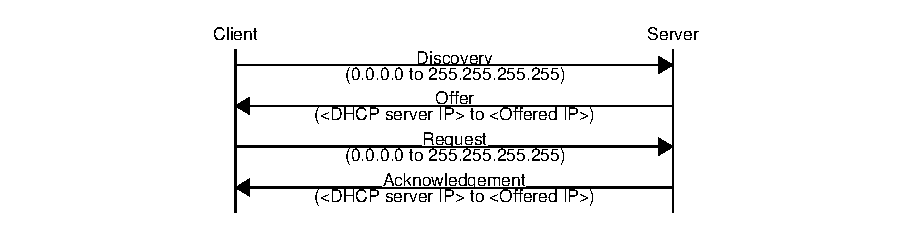
\includegraphics[width=\linewidth]{dhcp_dora.eps}
\end{center}


\begin{itemize}

\item \textbf{Discovery}\\
The goal of this message is to find DHCP servers willing to provide 
a configuration.\\[-0.3cm]

In the first communication, the client 
doesn't know the DHCP server's IP. Instead, it uses:
\begin{itemize}
\item Its MAC address as the source MAC address.
\item The LAN's broadcast (\otherBase{ff:ff:ff:ff:ff:ff}) as the destination MAC address.
\item \otherBase{0.0.0.0} as the source IP, meaning ``unknown''.
\item The \concept{local broadcast} address , \otherBase{255.255.255.255}, as the destination IP.
\end{itemize}

\vspace{0.25cm}
\item \textbf{Offer}\\
Zero or more servers will reply to the client with configuration offers.
These configurations (\eg, IP addresses) are not property of the client 
until the server sends a DHCP Acknowledgement.\\[-0.3cm]

The server keeps track of a \concept{pool} of addresses that dynamically 
assigns to clients.
% 
IP addresses are offered for a fixed period of time, after which they expire
unless they are \conceptRef{renew}{renewed} (see below). Addresses that are not renewed are put 
back in the pool and offered back to clients as they make requests.
\\[-0.3cm]

The server can use its real IP address and the one offered to the client.
The client knows it's the recipient because the server pays attention to the 
client's Discovery source MAC address.

\vspace{0.25cm}
\item \textbf{Request}\\
The client picks one of the received offers and requests that the 
assignment is completed.\\[-0.3cm]

The client uses the local broadcast
address, \otherBase{255.255.255.255}, as the destination and 
\otherBase{0.0.0.0} as the source: the offered address is still not the client's.

\vspace{0.25cm}
\item \textbf{Acknowledgement}\\
The server confirms the request. Once the client receives this ACK,
it starts using the offered configuration as its own. \\[-0.3cm]

It is also possible that the server denies the request, \eg, if 
too much time has passed since the offer. In this case, 
a negative Acknowledgement (NACK) is sent instead. If a NACK is received,
the client needs to go back to the Discover phase.
\end{itemize}

When a DHCP server \conceptRef{lease}{leases} an address to a client, it does 
so for a limited period of time $T$. This period is set by the DHCP server, and can be configured.
After $T/2$ is elapsed, clients may try to renew the leased configuration. To do so,
the Request-Acknowledgement cycle is repeated over time until either end fails to complete it in time,
or the DHCP server sends a NACK.

\begin{center}
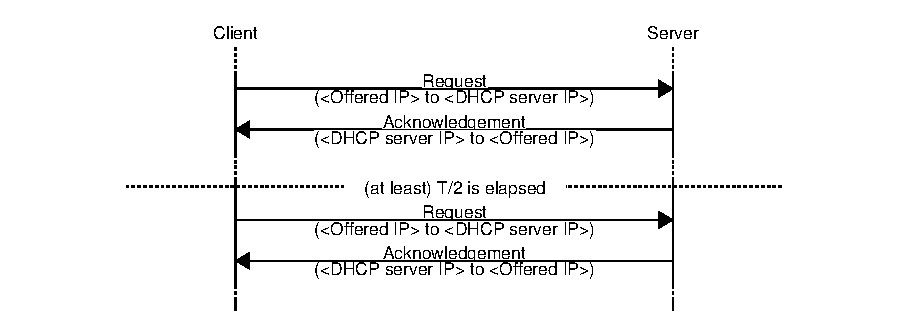
\includegraphics[width=\linewidth]{dhcp_renewal.eps}
\end{center}

\begin{exercise}
The typical domestic router implements both a DHCP client and a DHCP server.
Explain how this is possible and why it is useful.
\end{exercise}


\section{Autonomous Systems}

Routing is performed one \concept{hop} at a time, using \conceptRef{routing table}{routing tables} 
as discussed in Section~\ref{sec:layer3:routing}. Those tables need to be coordinated at a large 
scale to guarantee graph connectivity to all hosts in the Internet.


\subsection{Organization}

To facilitate this coordination, LANs are grouped in \conceptRef{autonomous system (AS)}{autonomous systems} (AS).
These are non-overlapping blocks of IP addresses (\otherBase{w.x.y.z/N}) that are separately owned and managed.
Many companies, universities and ISPs have their own ASs that are publicly 
\href{https://2ip.io/analytics/asn-list/}{\underline{listed}}. For instance, UAB's network belongs to
AS13041.

Each AS has to operate \conceptRef{border router}{border routers} (BR). When a border router receives a datagram 
with destination inside the AS, it forwards the datagram through the AS' \conceptRef{internal router}{internal routers} (IR).
Similarly, when a host inside an AS needs to contact a host in another AS, datagrams are forwarded through border routers
until they reach the destination AS and ultimately the destination LAN.

\begin{center}
  \vspace{-0.2cm}
 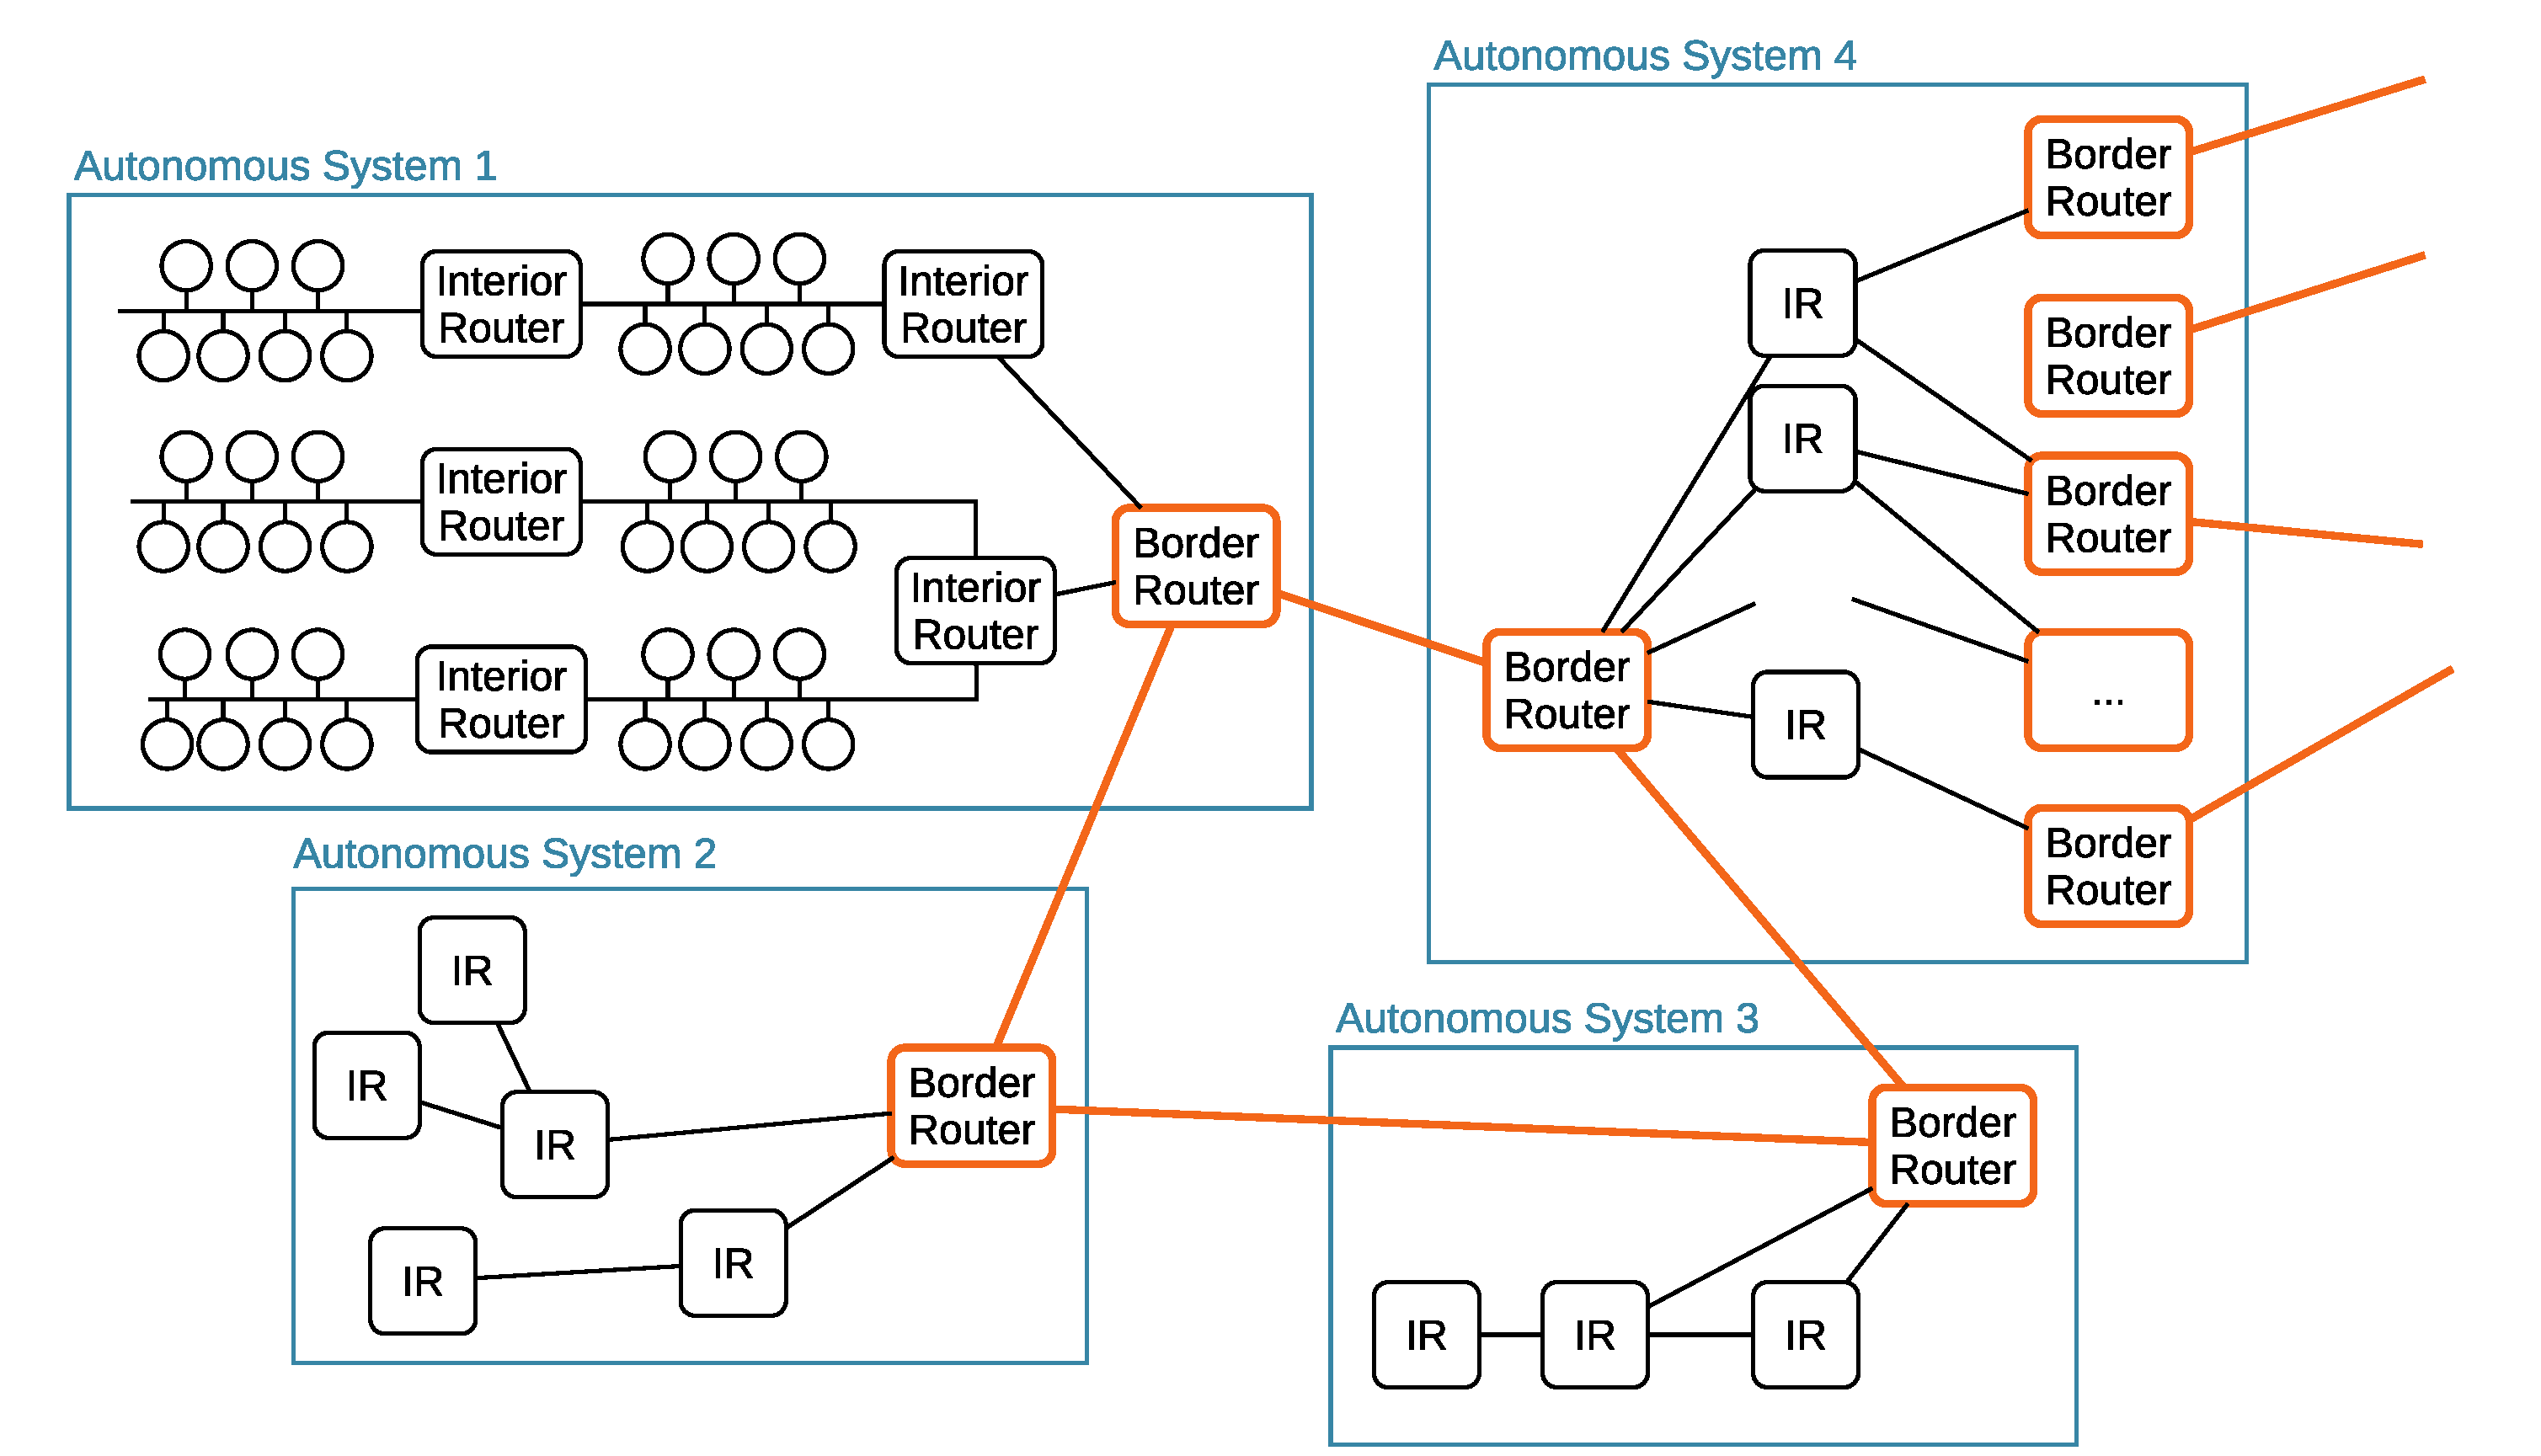
\includegraphics[width=\linewidth]{as.pdf}
 \vspace{-0.75cm}
\end{center}

\subsection{Routing table configuration}

Manually configuring the \conceptRef{routing table}{routing tables} of all border routers and internal routers
would be too costly and prone to errors. Instead, different algorithms are employed to configure them automatically.
\begin{itemize}
\item Within the AS, internal routers and border routers use one of the available 
\conceptRef{interior gateway protocol}{interior gateway protocols}.
Often, \concept{RIP} (Routing Information Protocol) is used due to its relatively simple configuration.
That said, ASs may freely choose the algorithm they use internally to their AS.\\[-0.2cm]

RIP implements a variation of the Bellman-Ford shortest path algorithm to minimize the number of \conceptRef{hop}{hops}
datagrams need to travel within the AS. Periodically (\eg, every $30$~s), each IR and BR:\\[-0.4cm]
% 
  \begin{enumerate}
  \item Advertises its \textit{perceived} distance to other routers in the AS.
  \item Updates its perceived distances based on other router's advertisements.
  \item Updates its \concept{routing table} to all LANs in the AS accordingly.
  \end{enumerate}

\begin{exercise}
RIP uses the number of hops as its cost metric.
% 
How could this be problematic?
% 
How can this problem be solved?
\end{exercise}

\vspace{0.25cm}
\item Between ASs, only border routers need be configured; interior routers simply need to direct 
exterior traffic through the border routers. \\[-0.3cm]

Border routers run an \concept{exterior gateway protocol} in addition to the 
interior gateway protocol used within the AS. Different ASs must agree on the 
algorithm they use, so \concept{BGP} (border gateway protocol) is normally used.\\[-0.3cm]

\concept{BGP} is a more complex protocol than \concept{RIP}. This complexity 
is needed because BGP coordinates border routers belonging to different ASs, \ie, 
with different owners:\\[-0.4cm]
\begin{itemize}
\item RIP uses a single number (the distance, \ie, the number of \conceptRef{hop}{hops})
to guide a shortest-path graph algorithm. BGP uses \conceptRef{path}{paths} instead of distances.
This allows BGP to choose routes with more \conceptRef{hop}{hops}, but more desirable to the AS,
\eg, in terms of time, monetary cost, internal load, etc.\\[-0.4cm]

\item BGP was designed with the notion of security and trust in mind, and includes mechanisms
to verify the authenticity of the paths announced by a border route.
\end{itemize}

\begin{exercise}
How can BGP translate economic interest into routing configurations?
\end{exercise}

\end{itemize}

\begin{remark}
BGP can also be used as the AS' interior gateway protocol. 
This is typically done only by very large ASs.
\end{remark}

% 
% - DHCP
% - Application protocols: HTTP, SMTP, IMAP
% - AS, rip/ospf
% 
% - capas TLS, compresión

% - client vs server (in TCP/IP, symmetry)?
% - server-client model
% - global structure, ownership and organization, 
